\subsection{Muon Fake Rate}
This section presents in more detail the studies on the muon fake rate.

\subsubsection{Fakeable Object}
The muon fakeable object definition is simply the muon selection requirements (Sec.~\ref{sec:sel_muons}) 
but with looser $d_0$ and isolation thresholds:
\begin{itemize}
  \item $|d_{0}| < 0.2$~cm
  \item $\frac{\rm{Iso}_{Total}}{\pt}~<~0.5$
\end{itemize}
Note that this has tighter isolation requirements than the definition studied in~\cite{fakeLeptonNote2}, 
which used $\rm{Iso}_{Total}/{\pt}~<~1.0$. The motivation for the tighter selection is the reduction of
systematic uncertainties by reducing the extrapolation in isolation.

\subsubsection{Calibration Sample Selection}
The muon fake rate has been measured in $5/ipb$ of data in Run2011A. The selected events are triggered
by any one of HLT\_Mu8 or HLT\_Mu15 single muon trigger paths. Addition requirements are also needed to
reduce contamination of the calibration sample with muons from $W$ and $Z$ decays and to tune the
jet composition:
\begin{itemize}
  \item $Z$ veto: reject the event if there are two oppositely charged muons satisfying the loose muon 
        selection and with $p_T>20\:\GeVc$,
  \item $W$ veto: reject the event if PF-MET $> 20\:\GeV$ or if the transverse mass of the loose muon 
        and PF-MET is above $20\:\GeVcc$,
  \item require the presence of a PF-jet with $p_T > 15\:\GeVc$ and separated by $\Delta R > 1$ 
        from the loose muon.
\end{itemize}
The jet threshold of $p_T > 15\:\GeVc$ was found to best model the jet spectrum of the $W+$jets process according to~\cite{fakeLeptonNote2}.
This needs to be verified in the 2011 data and Spring11 Monte Carlo samples.

\subsubsection{Fake Rates}
The fake rate parametrized in $\eta$-$p_T$ is listed in Tab.~\ref{tab:mu_fr_iso05_jet15}. Fig.~\ref{fig:mu_fr_iso05_jet15} shows
how the fake rate trends when projected onto $p_T$ or $\eta$.

\begin{table}[!htbp]
\begin{center}
\begin{tabular}{|c|c|c|c|c|c|}
\hline
  & $0<\eta<0.5$ & $0.5<\eta<1$ & $1<\eta<1.5$ & $1.5<\eta<2$ & $2<\eta<2.4$ \\
\hline 
$10 < p_T < 15$ & $0.1471 \pm 0.0073$ & $0.1684 \pm 0.0076$ & $0.1769 \pm 0.0075$ & $0.1934 \pm 0.0084$ & $0.2135 \pm 0.0141$ \\
\hline
$15 < p_T < 20$ & $0.1220 \pm 0.0033$ & $0.1330 \pm 0.0034$ & $0.1479 \pm 0.0038$ & $0.1664 \pm 0.0043$ & $0.1612 \pm 0.0079$ \\
\hline
$20 < p_T < 25$ & $0.1900 \pm 0.0083$ & $0.2265 \pm 0.0089$ & $0.2398 \pm 0.0090$ & $0.2542 \pm 0.0102$ & $0.2828 \pm 0.0189$ \\
\hline
$25 < p_T < 30$ & $0.2008 \pm 0.0155$ & $0.2306 \pm 0.0165$ & $0.2056 \pm 0.0167$ & $0.2763 \pm 0.0198$ & $0.2694 \pm 0.0357$ \\
\hline
$30 < p_T < 35$ & $0.1565 \pm 0.0241$ & $0.1786 \pm 0.0259$ & $0.2427 \pm 0.0309$ & $0.2913 \pm 0.0351$ & $0.3750 \pm 0.0699$ \\
\hline
$35 < p_T < 40$ & $0.2895 \pm 0.0487$ & $0.2222 \pm 0.0498$ & $0.2923 \pm 0.0453$ & $0.2289 \pm 0.0555$ & $0.3333 \pm 0.1142$ \\
\hline
\end{tabular}
\caption{Muon fake rate in $\eta$-$p_T$. Uncertainties are statistical only.}
\label{tab:mu_fr_iso05_jet15}
\end{center}
\end{table}

\begin{figure}[!htbp]
\begin{center}
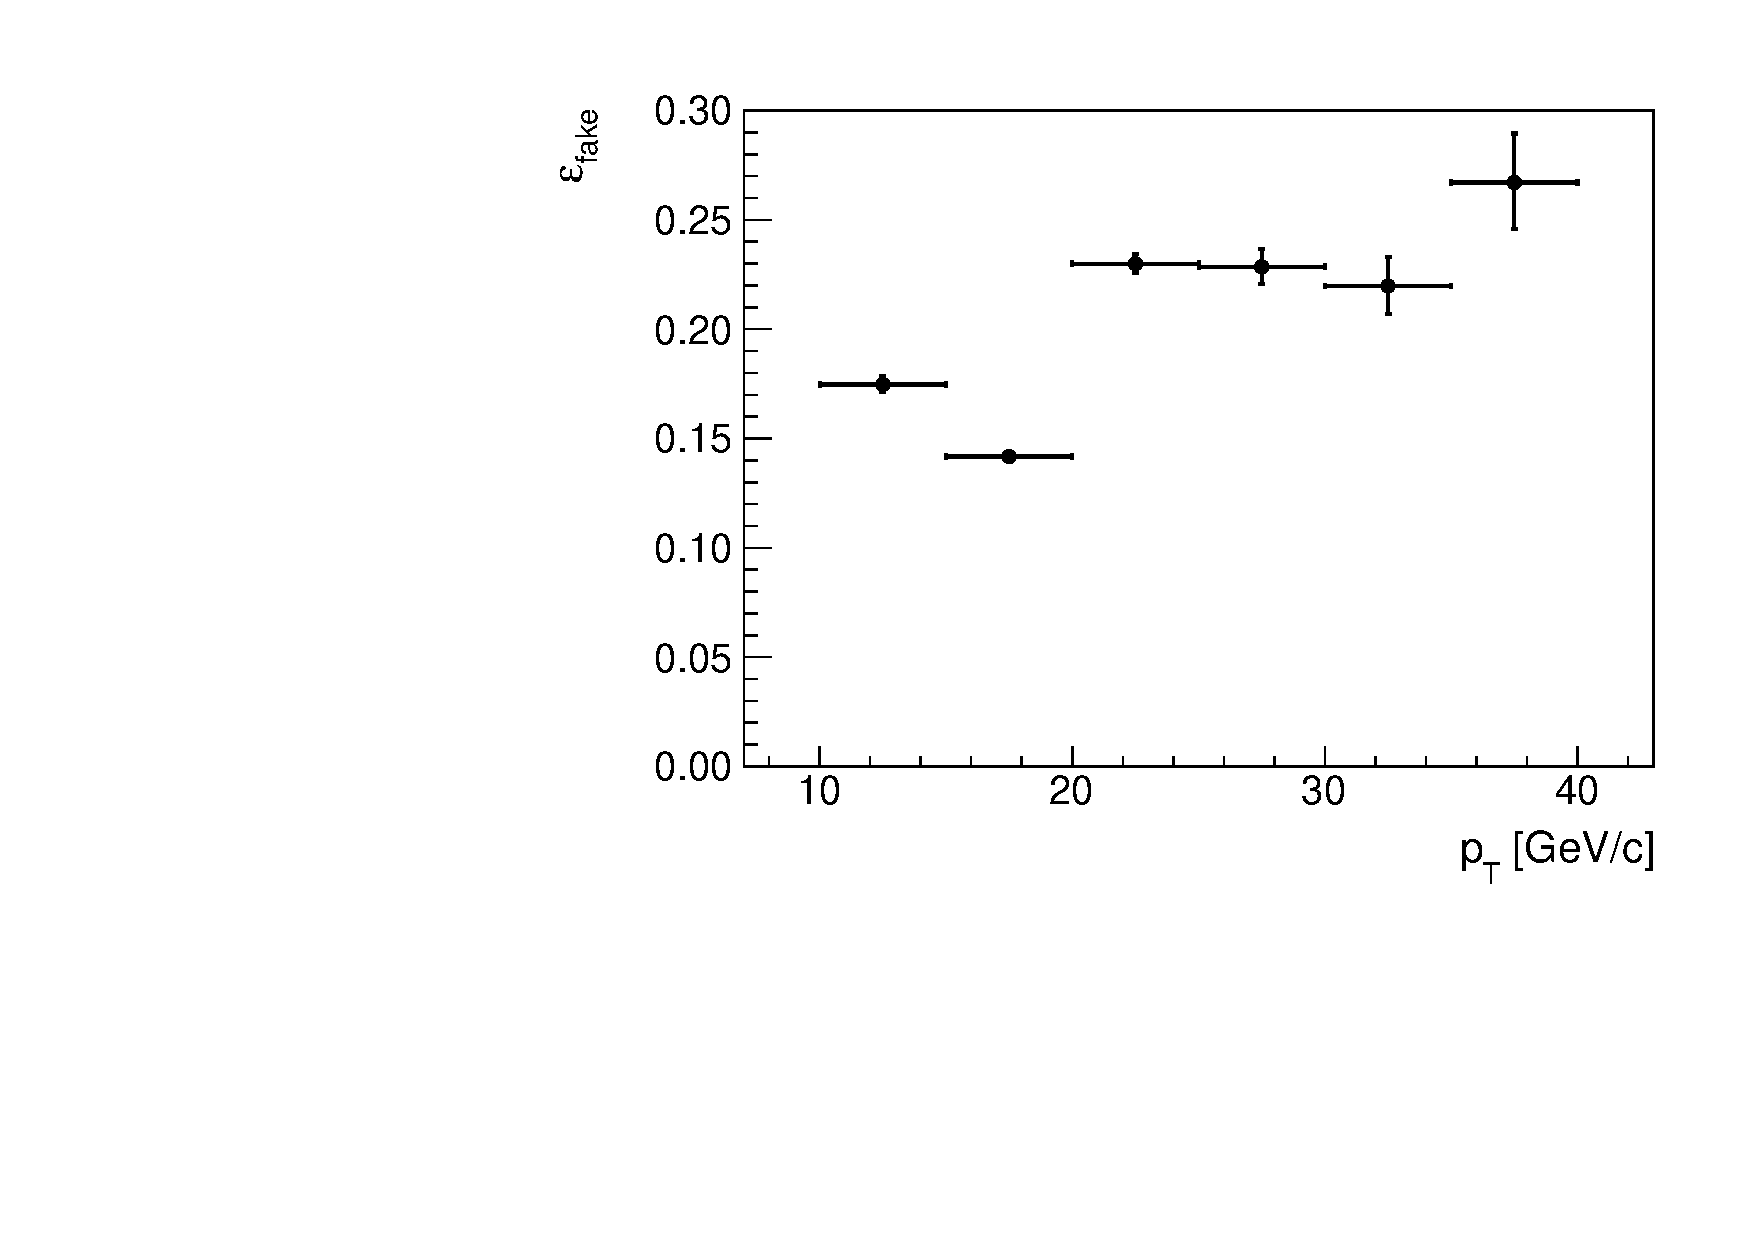
\includegraphics[width=0.45\textwidth]{figures/muon_frpt.pdf}
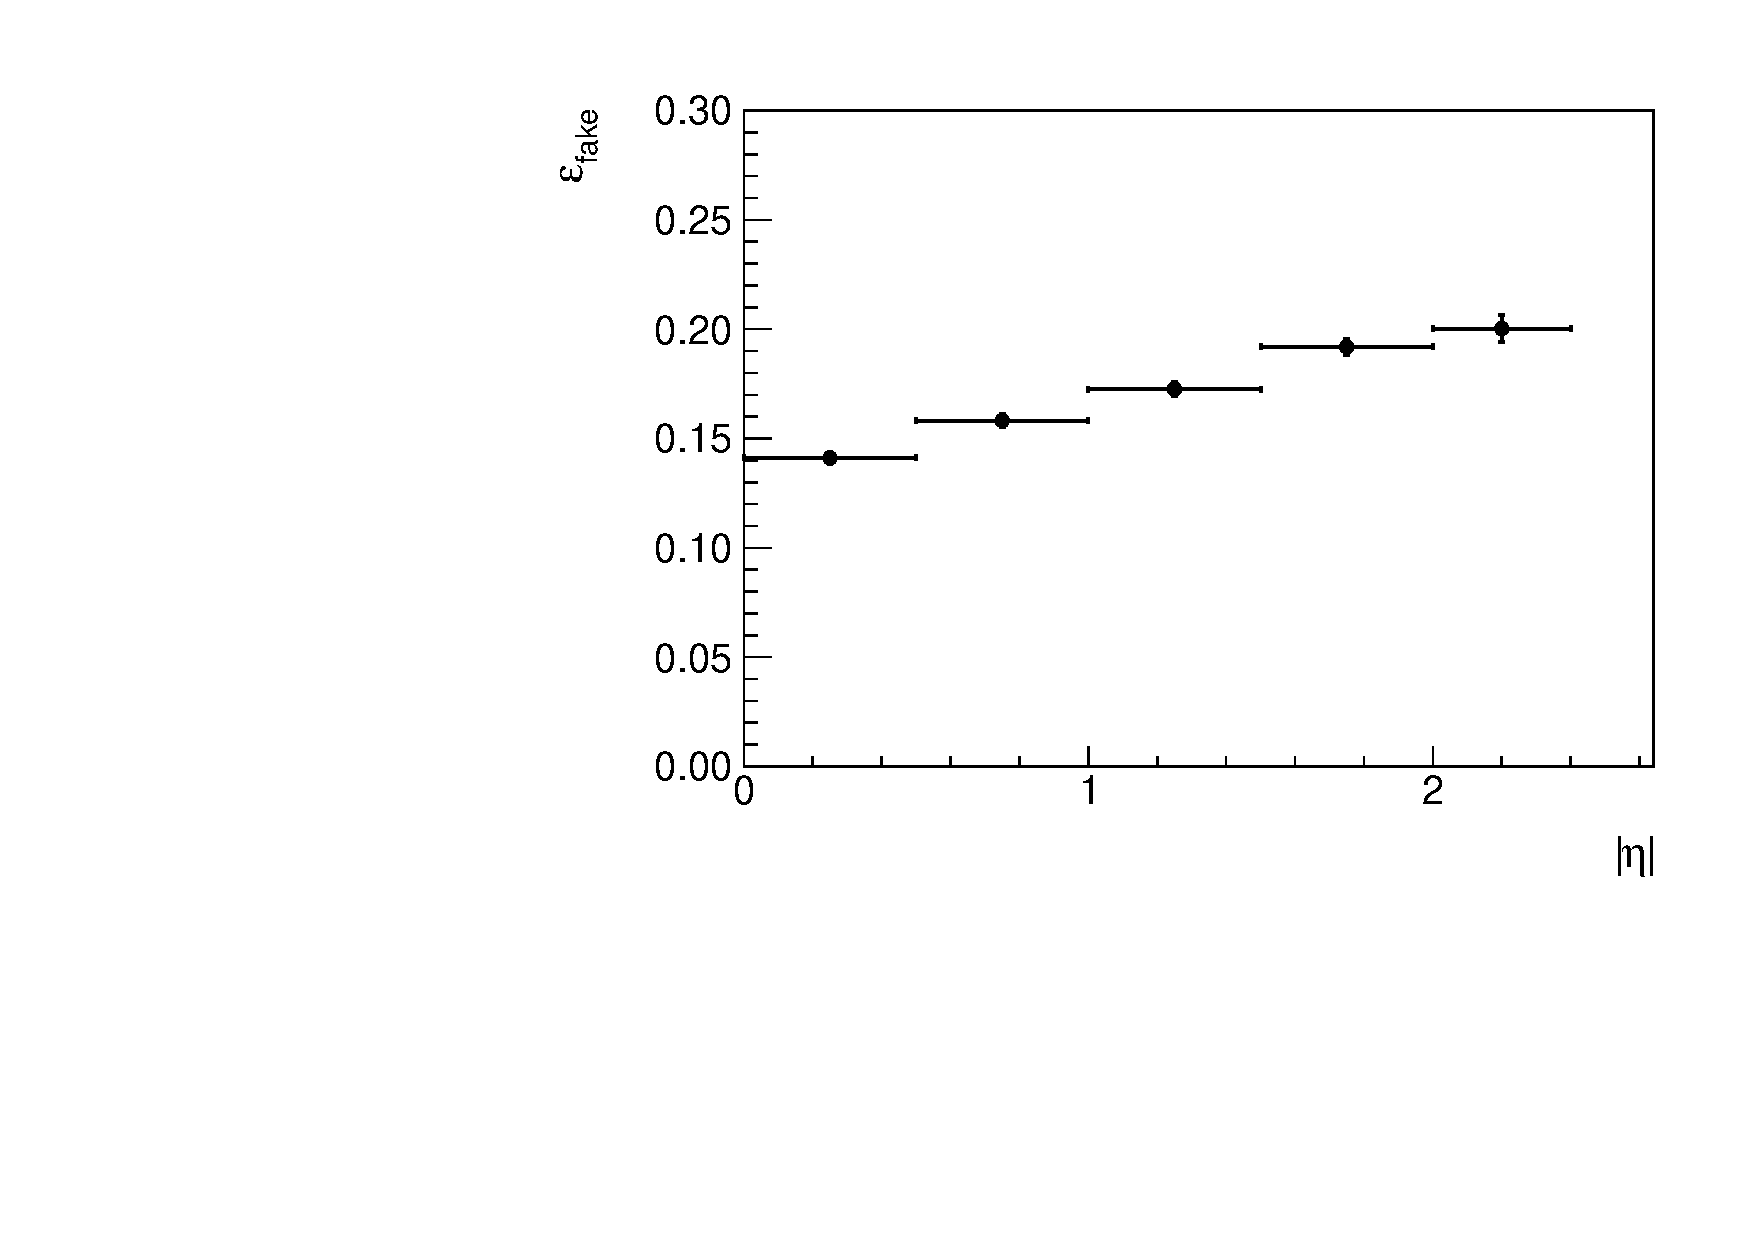
\includegraphics[width=0.45\textwidth]{figures/muon_freta.pdf}
\caption{Fake rates projected onto $p_T$ and $\eta$.}
\label{fig:mu_fr_iso05_jet15}
\end{center}
\end{figure}

\subsubsection{Sample Dependence}
The systematic uncertainty associated with the jet sample dependence is estimated by measuring the difference in the
fake rate when the jet threshold is changed. In addition to the standard calibration sample defined previously, we
also measure the fake rate in a sample defined by a jet $p_T>30\:\GeVc$ threshold and in a sample without a jet
requirement. The largest difference from the nominal fake rate is taken as the systematic uncertainty. The fake rate
projections onto $p_T$ and $\eta$ for various jet requirements are shown in Fig.~\ref{fig:mu_fr_iso05}. The systematic
uncertainties are $34\%$ for $p_T<20\:\GeVc$, $20\%$ for $p_T>20\:\GeVc$, and $23\%$ overall. In contrast, the definition
used in~\cite{fakeLeptonNote2} yields systematic uncertainties of $46\%$ for $p_T<20\:\GeVc$, $29\%$ for $p_T>20\:\GeVc$, 
and $36\%$ overall.

\begin{figure}[!htbp]
\begin{center}
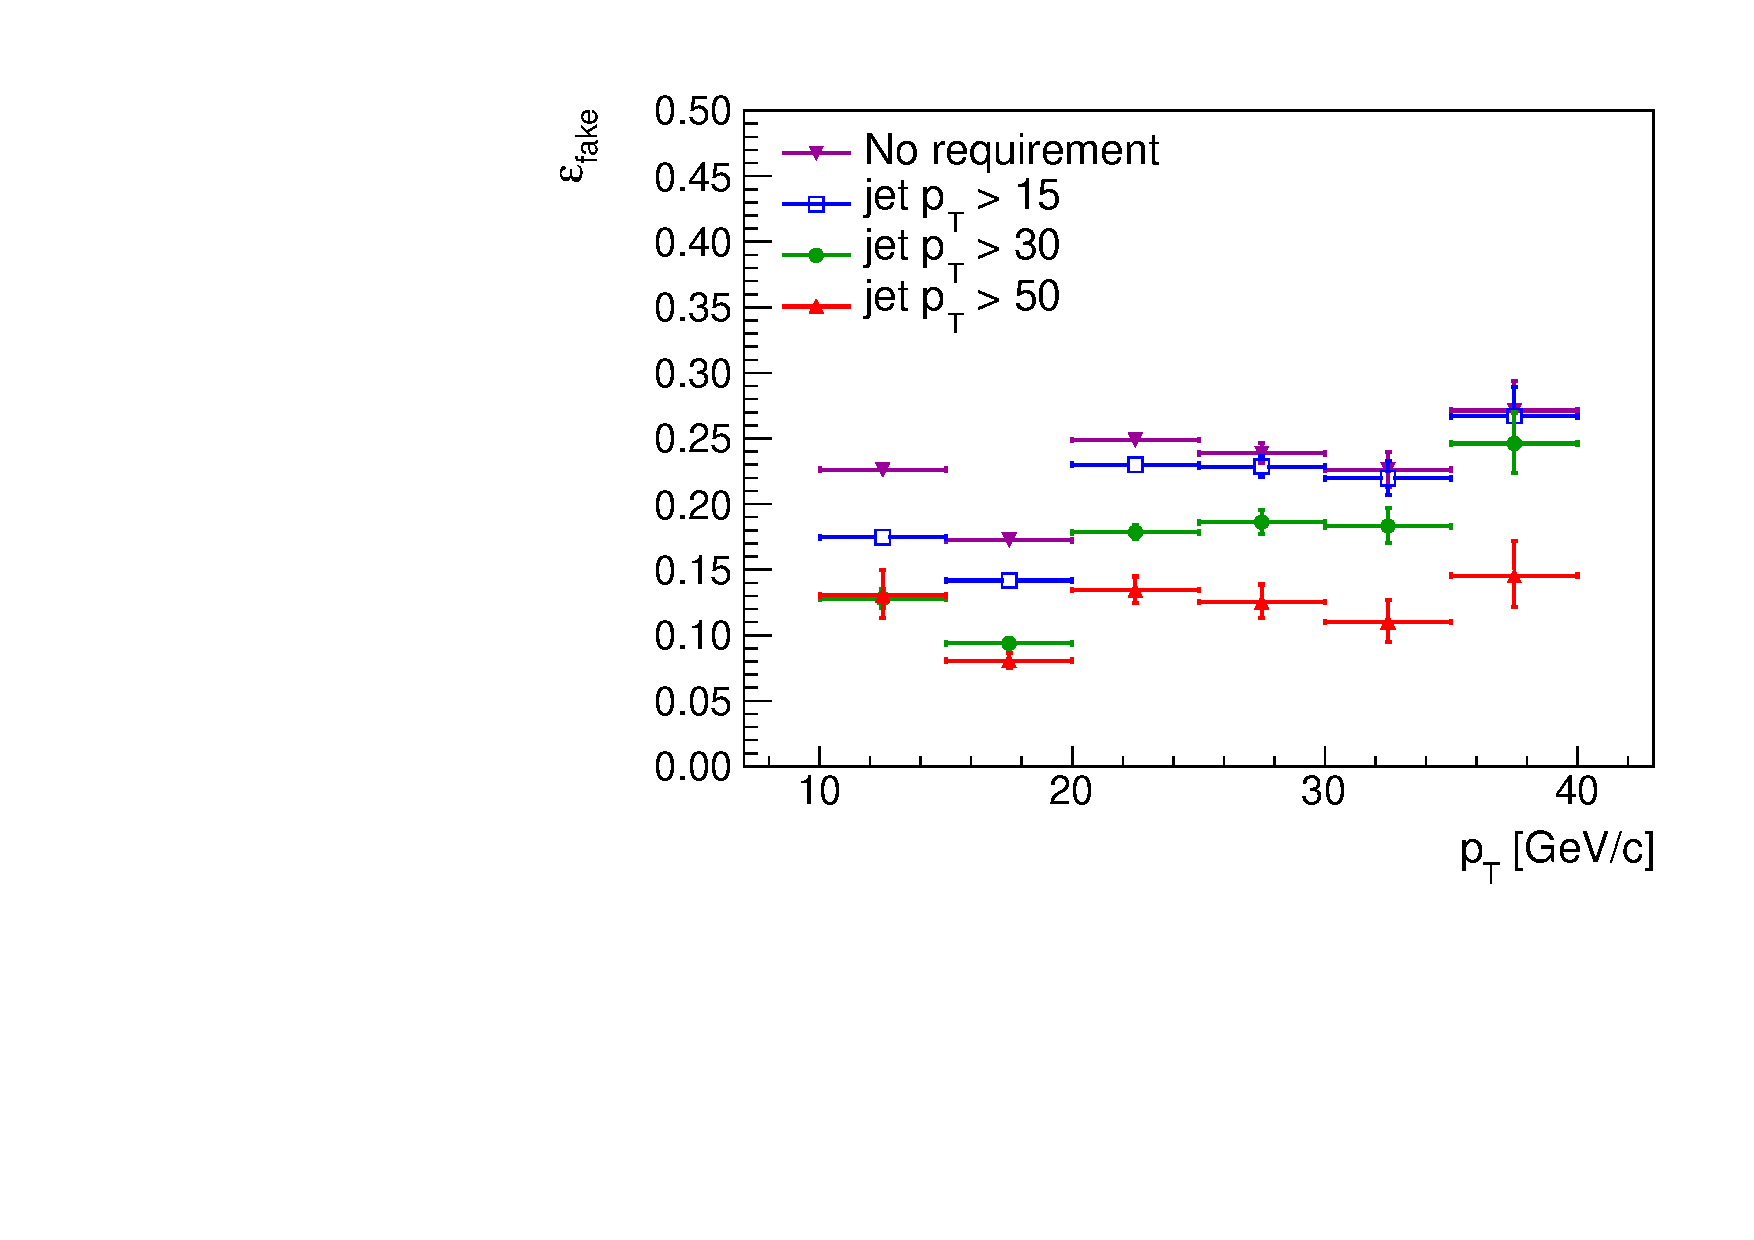
\includegraphics[width=0.45\textwidth]{figures/muon_frpt_jetscan.pdf}
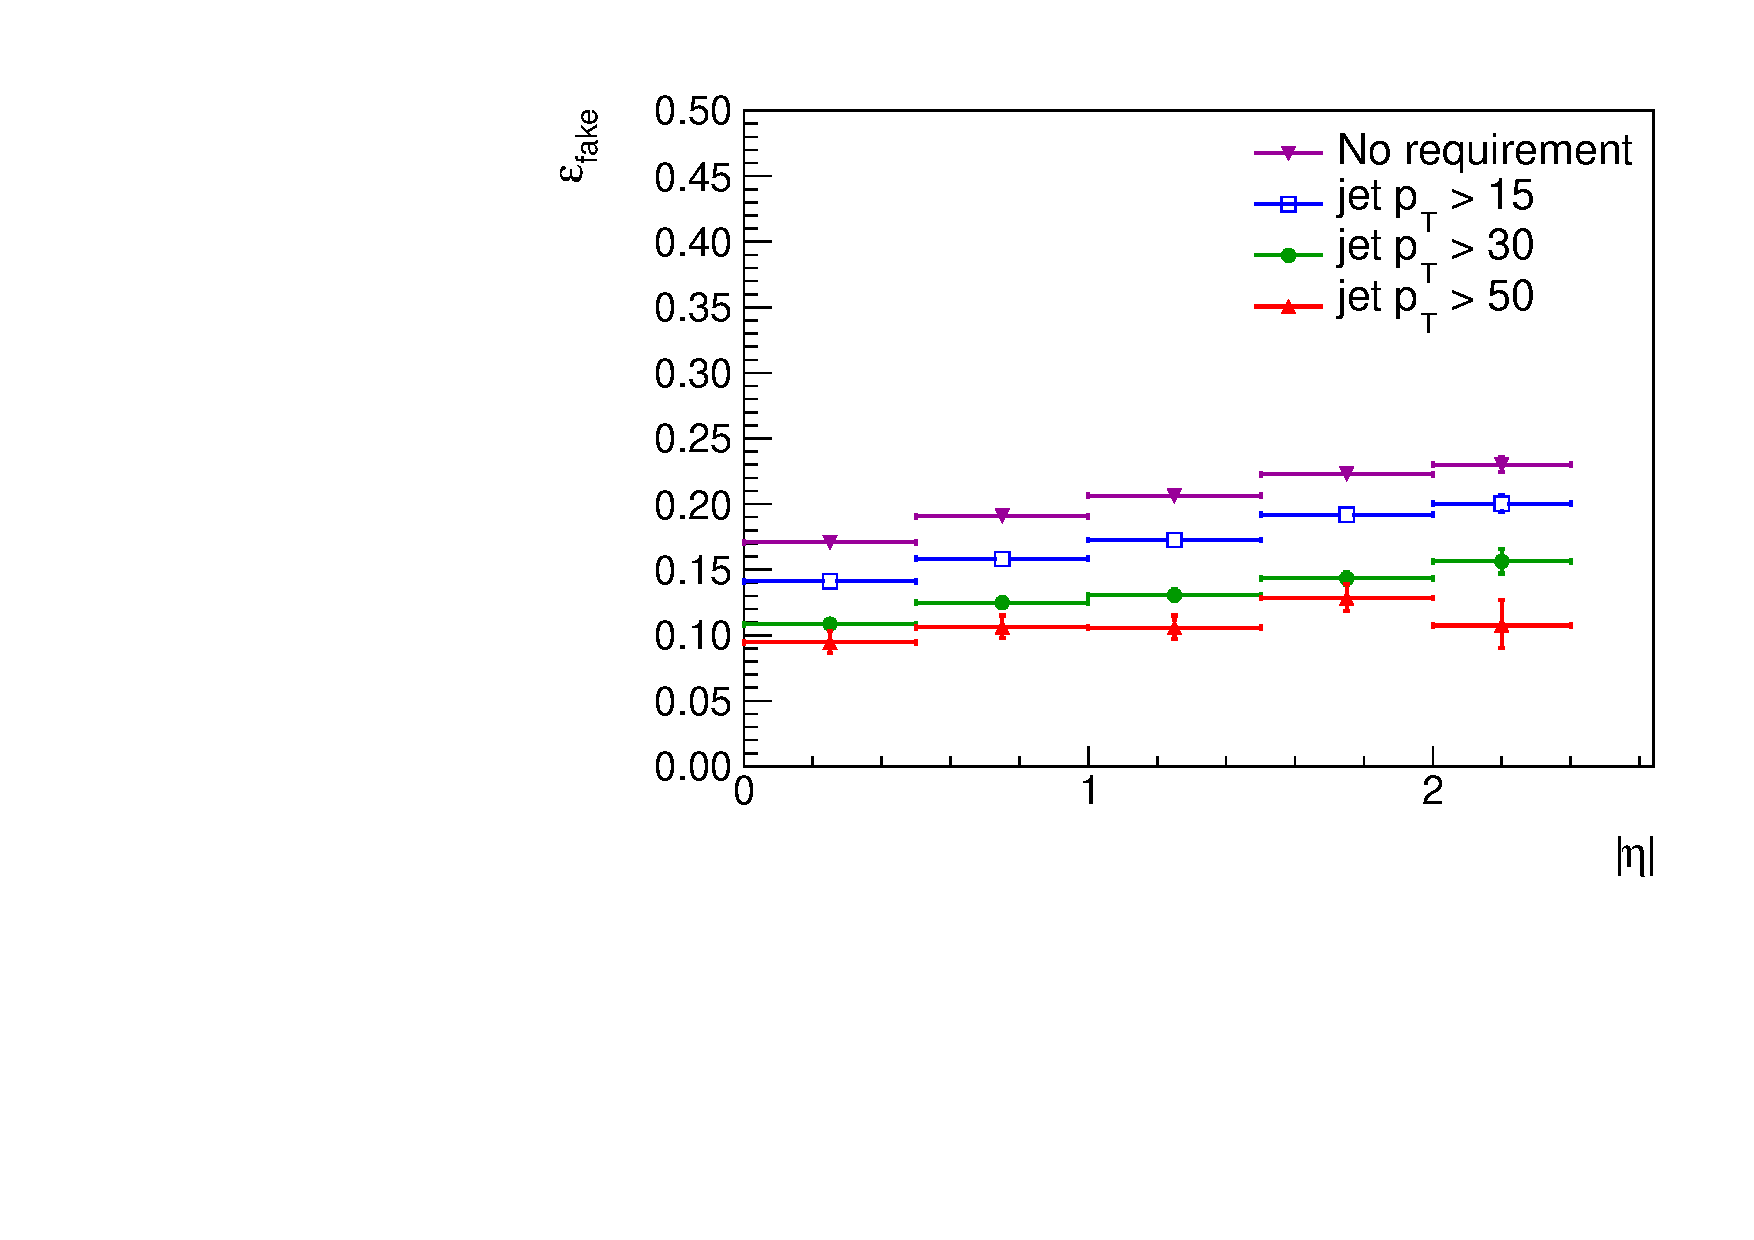
\includegraphics[width=0.45\textwidth]{figures/muon_freta_jetscan.pdf}
\caption{Fake rates projected onto $p_T$ and $\eta$.}
\label{fig:mu_fr_iso05}
\end{center}
\end{figure}
